\chapter{Apparecchi di manovra, protezione e relè}
Gli apparecchi di manovra e protezione costituiscono i componenti fondamentali per la gestione dell'esercizio, la riconfigurazione e la salvaguardia dei sistemi elettrici di potenza sia in condizioni ordinarie che in presenza di anomalie o guasti.

Un apparecchio di manovra è un dispositivo capace di svolgere almeno una delle seguenti funzioni:
\begin{enumerate}
    \item Interrompere la corrente in un circuito elettrico.
    \item Stabilire la corrente in un circuito elettrico.
\end{enumerate}

Le manovre di apertura e chiusura possono effettuarsi in due differenti condizioni operative della rete:
\begin{itemize}
    \item \textbf{Condizioni normali del circuito elettrico (circuito "sano")} $\rightarrow$ quando nel circuito circola la corrente di normale funzionamento (corrente nominale o di carico) oppure una corrente di sovraccarico.
    \item \textbf{Condizioni anormali del circuito elettrico (circuito "guasto")} $\rightarrow$ quando nel circuito circola la corrente di cortocircuito.
\end{itemize}

\section{Classificazione degli apparecchi di manovra}
Gli apparecchi di manovra si suddividono in:
\begin{itemize}
    \item \textbf{Sezionatori} $\rightarrow$ costruiti per aprire o chiudere, in modo visibile o mediante un dispositivo indicatore affidabile, un circuito percorso da correnti di intensità trascurabile (es. per dare certezza all'operatore che il circuito sia disalimentato e isolato).
    \begin{figure}[H]
    	\centering
    	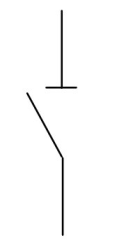
\includegraphics[width=0.07\linewidth]{immagini/manovra}
    \end{figure}
    \item \textbf{Interruttori} $\rightarrow$ costruiti per aprire o chiudere un circuito percorso da correnti di intensità non trascurabile, comprese quelle elevate di cortocircuito.
    \begin{figure}[H]
    	\centering
    	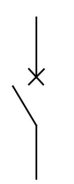
\includegraphics[width=0.06\linewidth]{immagini/manovra1}
    \end{figure}
    \item \textbf{Interruttori di manovra} $\rightarrow$ costruiti per aprire un circuito esclusivamente in condizioni normali (corrente nominale e di sovraccarico) o per chiudere un circuito sia in condizioni normali che anormali (anche su cortocircuito).
    \begin{figure}[H]
    	\centering
    	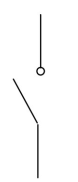
\includegraphics[width=0.06\linewidth]{immagini/manovra2}
    \end{figure}
    \item \textbf{Interruttori di manovra-sezionatori} $\rightarrow$ interruttori di manovra per i quali deve essere possibile verificare la posizione di contatto aperto in modo visibile o mediante un dispositivo indicatore affidabile.
    \begin{figure}[H]
    	\centering
    	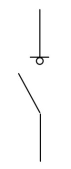
\includegraphics[width=0.06\linewidth]{immagini/manovra3}
    \end{figure}
    \item \textbf{Contattori} $\rightarrow$ costruiti per aprire o chiudere un circuito esclusivamente in condizioni normali.
    \begin{figure}[H]
    	\centering
    	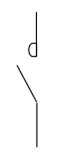
\includegraphics[width=0.06\linewidth]{immagini/manovra4}
    \end{figure}
    \item \textbf{Fusibili} $\rightarrow$ apparecchi privi di contatti mobili convenzionali che interrompono automaticamente circuiti a media e bassa tensione mediante la fusione di una parte calibrata quando la corrente supera un valore prefissato per un tempo sufficiente.
    \begin{figure}[H]
    	\centering
    	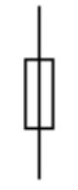
\includegraphics[width=0.06\linewidth]{immagini/manovra5}
    \end{figure}
\end{itemize}

Di seguito sono riassunte le funzioni dei principali apparecchi di manovra:
\begin{figure}[H]
	\centering
	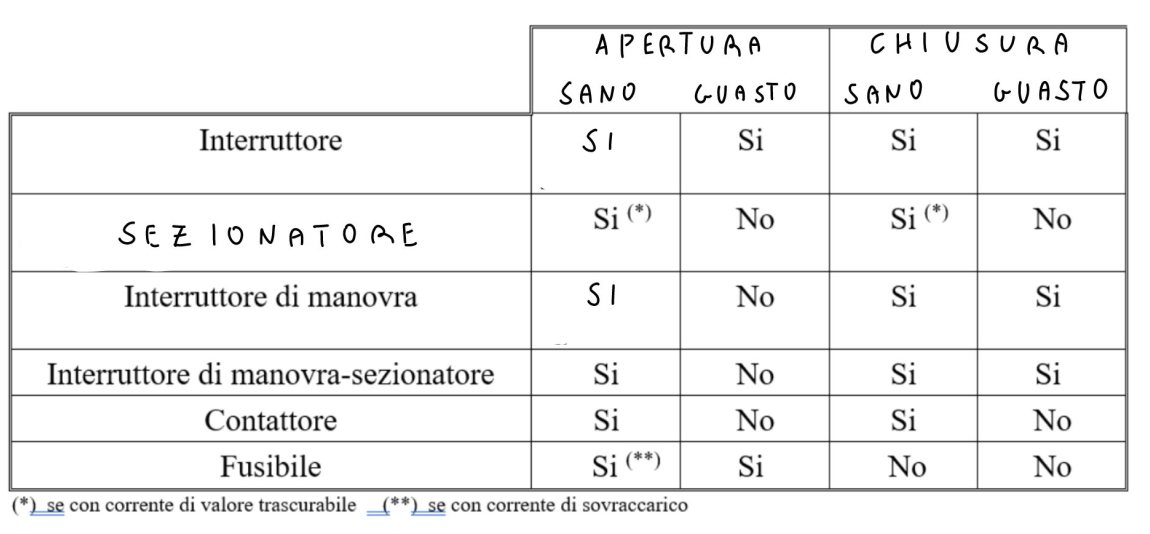
\includegraphics[width=0.8\linewidth]{immagini/manovra6}
\end{figure}

\section{Apertura di un circuito e arco elettrico}
In un interruttore sono presenti due contatti conduttori (uno fisso e uno mobile) che vengono allontanati tramite opportuni comandi o sganciatori quando si richiede l'apertura del circuito.

Il distacco meccanico dei contatti non è seguito istantaneamente dall'estinzione della corrente: la corrente continua a fluire nello spazio per un certo lasso di tempo a causa della formazione di un \textbf{arco elettrico}.
\begin{figure}[H]
	\centering
	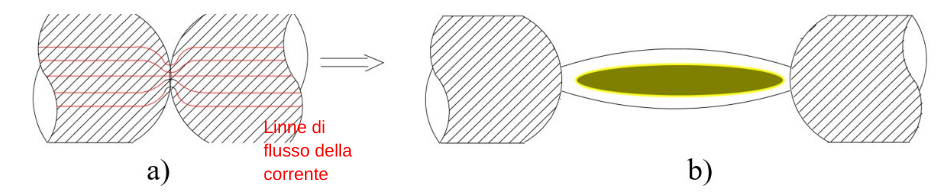
\includegraphics[width=0.7\linewidth]{immagini/manovra7}
\end{figure}
La sequenza fisica dell'apertura si sviluppa secondo i seguenti passaggi:
\begin{enumerate}
    \item I contatti elettrici vengono progressivamente allontanati dai meccanismi di sgancio.
    \item La superficie o sezione utile di contatto metallico al passaggio della corrente si riduce drasticamente a pochi punti di contatto microscopici.
    \item La resistenza localizzata di contatto aumenta considerevolmente per la costrizione delle linee di flusso della corrente.
    \item Aumentano localmente le perdite per effetto Joule e la temperatura dei punti di contatto.
    \item Si un arco elettrico, che conduce corrente, opponendosi alla discontinuità introdotta dalla separazione meccanica dei contatti.
\end{enumerate}

La modalità di estinzione dell'arco si differenzia radicalmente in funzione della natura della corrente:
\begin{itemize}
    \item \textbf{Corrente alternata (AC)} $\rightarrow$ la corrente attraversa periodicamente e naturalmente il valore zero (due volte per ciclo). L'annullarsi periodico della corrente determina uno spegnimento "naturale" dell'arco. Il problema tecnologico primario dell'interruzione in alternata consiste nell'evitare che l'arco si riadeschi di nuovo.
    \item \textbf{Corrente continua (DC)} $\rightarrow$ non si ha alcun passaggio naturale per lo zero della corrente. L'interruzione deve essere forzata "innaturalmente" introducendo una resistenza d'arco sufficientemente elevata da abbattere la corrente fino all'annullamento; tale risultato si ottiene allungando l'arco.
\end{itemize}

\newpage
\section{Interruttori}
L'interruttore è l'apparecchio di manovra e protezione progettato per stabilire, sopportare e interrompere correnti in tutte le condizioni di esercizio, incluse le correnti di cortocircuito massime presunte nel punto di installazione.

\subsection{Introduzione al cortocircuito}
Per comprendere i requisiti prestazionali richiesti a un interruttore, la porzione di rete a monte del guasto può essere schematizzata mediante un circuito equivalente $RL$ serie alimentato da una sorgente sinusoidale di tensione $e(t) = \sqrt{2} E \sin(\omega t + \alpha)$.
\begin{figure}[H]
	\centering
	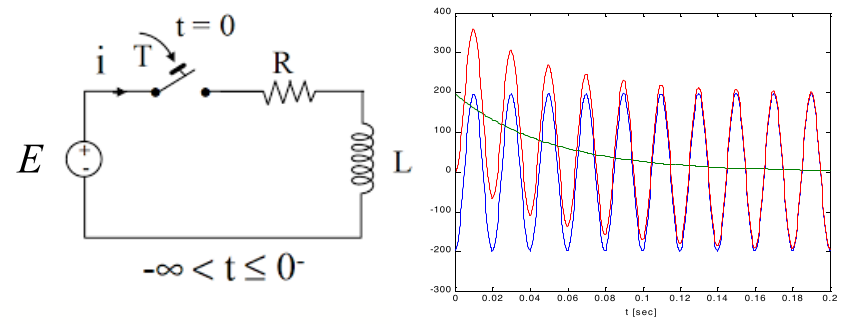
\includegraphics[width=0.8\linewidth]{immagini/manovra9}
\end{figure}
\[i(t) = i_p(t) + i_t(t) = \sqrt{2} I_k \sin(\omega t + \alpha - \varphi) - \sqrt{2} I_k \sin(\alpha - \varphi) e^{-\frac{t}{\tau}}\]
dove:
\begin{itemize}
    \item $i_p(t)$ $\rightarrow$ componente a regime della corrente di cortocircuito.
    \item $i_t(t)$ $\rightarrow$ componente transitoria a decadimento esponenziale, con costante di tempo $\tau = L/R$.
    \item $\alpha$ $\rightarrow$ angolo di fase della tensione all'istante di innesco del cortocircuito (variabile aleatoria legata all'evento del guasto).
    \item $\varphi$ $\rightarrow$ angolo di fase dell'impedenza di corto $\bar{Z} = R + j\omega L$, pari a $\varphi = \arctan(\omega L / R)$.
    \item $I_k = \frac{E}{Z}$ $\rightarrow$ valore efficace della componente a regime.
\end{itemize}

L'entità della componente transitoria dipende dalla fase all'innesco del guasto:
\begin{itemize}
    \item Se $\alpha = \varphi$ $\rightarrow$ la componente esponenziale è nulla; la corrente si assesta immediatamente a regime.
    \item Se $\alpha - \varphi = \pm \frac{\pi}{2}$ $\rightarrow$ la componente esponenziale assume la massima ampiezza iniziale possibile ($\pm \sqrt{2} I_k$), generando la condizione di cortocircuito asimmetrico più gravosa per l'impianto.
\end{itemize}

\textbf{VERIFICARE LE AFFERMAZIONI SEGUENTI:}\\
Il picco massimo della corrente di cortocircuito, indicato con $I_p$, si manifesta circa mezzo periodo dopo l'inizio del guasto:
\[I_p \approx \sqrt{2} \kappa I_k\]
con $\kappa$ fattore di cresta compreso tra $1$ e $2$ in funzione del rapporto $X/R$. Per il dimensionamento dell'apparecchiatura si considera tassativamente lo scenario peggiore (worst case).

\newpage
\subsection{Grandezze caratteristiche degli interruttori}
Il costruttore definisce l'attitudine operativa dell'interruttore mediante parametri normalizzati:
\begin{itemize}
    \item \textbf{Potere di apertura} $\rightarrow$ valore efficace della più elevata componente simmetrica (a regime) della corrente di cortocircuito \underline{presunta} che l'interruttore è in grado di interrompere, a una tensione specificata, qualunque sia il valore della componente unidirezionale (transitoria).
    \item \textbf{Potere di chiusura} $\rightarrow$ valore massimo della più elevata corrente di cortocircuito \underline{presunta} che l'interruttore è in grado di stabilire.
\end{itemize}

\textbf{Definizione di corrente di cortocircuito presunta:}
l'intervento dell'interruttore modifica spontaneamente la forma d'onda della corrente a causa della resistenza non lineare introdotta dall'arco elettrico e dall'estinzione anticipata della corrente rispetto al regime naturale. Per svincolare le specifiche dell'apparecchio dalla specifica risposta d'arco, si definisce come \emph{corrente presunta di cortocircuito} la corrente che circolerebbe nella rete qualora l'interruttore fosse sostituito da un conduttore di impedenza trascurabile (cortocircuito ideale). Essa rappresenta il caso limite ideale privo della resistenza smorzante dell'arco.

Nel primo caso si fa riferimento al \textbf{valore efficace} perché l’interruzione è
legata all’energia associata all’arco elettrico. Al contrario, il potere di chiusura è specificato in \textbf{valore massimo (picco)} perché questo è legato agli sforzi elettrodinamici che si generano tra i contatti (la forza per unire i contatti che è proporzionale al picco).

Durante una manovra di chiusura su un circuito accidentalmente in cortocircuito, prima del contatto metallico finale scocca un arco di pre-adescamento: le conseguenti forze repulsive tendono a respingere i contatti mobili, riducendone la velocità di chiusura e la pressione di contatto. Ne consegue un sensibile aumento dell'energia d'arco e della resistenza di contatto superficiale; in assenza di organi di comando dotati di forza sufficiente, si rischia la saldatura dei contatti o l'esplosione distruttiva dell'apparecchio.

\subsection{Intervalli temporali di manovra}
Le manovre di apertura e chiusura sono caratterizzate da intervalli temporali specifici:
\begin{itemize}
    \item \textbf{Tempo di apertura} $\rightarrow$ intervallo temporale che intercorre tra l'istante in cui viene applicato il comando di scatto al dispositivo di apertura e l'istante in cui i contatti principali iniziano a separarsi con lo scocco dell'arco.
    \item \textbf{Durata d'arco} $\rightarrow$ intervallo temporale tra l'istante di innesco dell'arco sui contatti e l'istante della sua definitiva e completa estinzione.
    \item \textbf{Tempo di interruzione} $\rightarrow$ intervallo complessivo pari alla somma del tempo di apertura e della durata d'arco.
    \item \textbf{Tempo di chiusura} $\rightarrow$ intervallo di tempo compreso tra l'istante in cui viene inviato il comando di chiusura e l'istante in cui si verifica il congiungimento metallico dei contatti in tutti i poli.
\end{itemize}

Poiché la maggioranza dei guasti sulle linee elettriche aeree è di tipo transitorio o fuggitivo (ad esempio scariche atmosferiche su isolatori), gli interruttori sono equipaggiati con dispositivi di richiusura automatica:
\begin{enumerate}
    \item All'atto del guasto l'interruttore scatta e apre il circuito.
    \item Dopo un tempo di attesa molto breve (richiusura rapida, circa $0{,}3\text{ s}$) l'interruttore si richiude automaticamente. Se il guasto è transitorio, l'alimentazione riprende senza disservizio prolungato.
    \item Se il guasto persiste, l'interruttore si riapre immediatamente; in alcuni impianti si attende un intervallo di tempo maggiore (richiusura lenta, da $1$ a $3\text{ minuti}$) e si effettua un secondo tentativo di chiusura.
    \item Se anche alla seconda richiusura il guasto risulta presente, il blocco interviene decretando l'apertura definitiva (apertura permanente) per l'isolamento del guasto stabile.
\end{enumerate}

Negli interruttori per tensioni superiori a $1000\text{ V}$, i valori nominali del potere di apertura e chiusura sono correlati a un ciclo di manovre normalizzato rappresentato dalla sequenza:
\[\text{O} - t - \text{CO} - t' - \text{CO}\]
dove:
\begin{itemize}
    \item $\text{O}$ $\rightarrow$ manovra di apertura.
    \item $\text{CO}$ $\rightarrow$ manovra di chiusura seguita immediatamente da una riapertura in caso sia ancora presente il guasto.
    \item $t, t'$ $\rightarrow$ tempi di attesa tra manovre consecutive (tipicamente $t = 0{,}3\text{ s}$ per richiusura rapida o $t = 3\text{ min}$ negli altri casi; $t' = 1\text{ min}$ o $t' = 3\text{ min}$).
\end{itemize}

\subsection{Tipologie costruttive degli interruttori}
Gli interruttori si classificano in base al mezzo dielettrico impiegato nella camera di estinzione per smorzare e raffreddare l'arco:
\begin{itemize}
    \item Interruttori in aria a pressione atmosferica.
    \item Interruttori in olio.
    \item Interruttori in aria compressa.
    \item Interruttori in esafluoruro di zolfo ($\text{SF}_6$).
    \item Interruttori sotto vuoto.
\end{itemize}

\subsubsection{Interruttori in aria a pressione atmosferica}
L'arco scocca e si estingue nell'aria ambiente a pressione atmosferica. 
\begin{figure}[H]
	\centering
	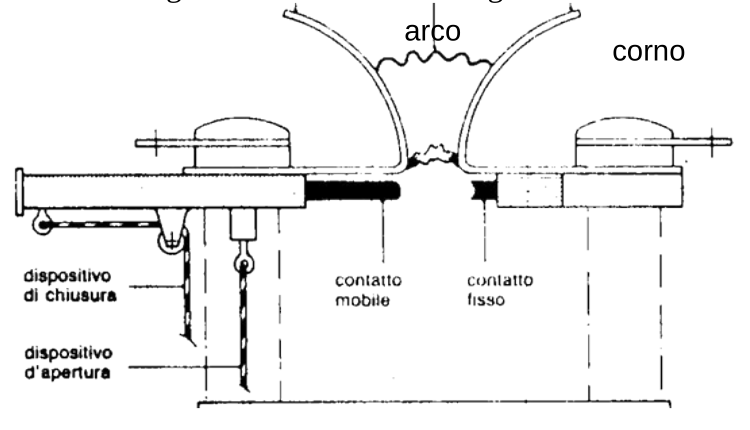
\includegraphics[width=0.5\linewidth]{immagini/manovra10}
\end{figure}
Il principio di funzionamento si basa su due azioni concorrenti:
\begin{enumerate}
    \item Quando il contatto mobile lascia il contatto fisso, si crea l'arco elettrico che si trasferisce per effetto
    termico sulle corna disposte superiormente. L’arco e le corna formano assieme un campo magnetico che
    interagendo con la corrente che percorre l’arco causa un’azione ponderomotrice che trasla l’arco verso
    l’alto. Il conseguente aumento della lunghezza dell'arco è tale da garantire lo spegnimento dello stesso.
    \item La conformazione dei contatti è studiata in modo che le correnti di cortocircuito scorrano in versi antiparalleli. Si sviluppa una forza repulsiva di natura elettrodinamica che si va a sommare a quella di natura meccanica e che accelera la separazione dei contatti.
\end{enumerate}
\begin{figure}[H]
	\centering
	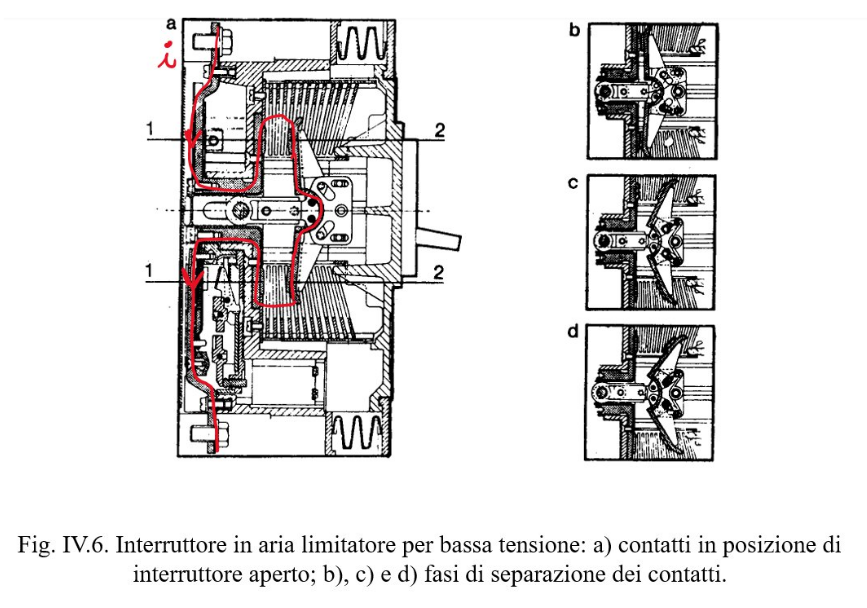
\includegraphics[width=0.7\linewidth]{immagini/manovra11}
\end{figure}

\subsubsection{Interruttori in esafluoruro di zolfo ($\text{SF}_6$)}
L'esafluoruro di zolfo è un gas dielettrico ampiamente impiegato nelle reti di media, alta e altissima tensione per le sue proprietà chimico-fisiche:
\begin{itemize}
    \item \textbf{Elevata rigidità dielettrica} $\rightarrow$ determinata dalle grandi dimensioni e dalla massa della molecola $\text{SF}_6$, che favoriscono urti anelastici capaci di rallentare e dissipare l'energia cinetica degli elettroni liberi (dell'arco elettrico) accelerati dal campo elettrico.
    \item \textbf{Elevato potere deionizzante} $\rightarrow$ grazie alla forte affinità elettronica degli atomi di fluoro, l'$\text{SF}_6$ cattura con eccezionale prontezza gli elettroni liberi della scarica formando ioni negativi pesanti e a ridottissima mobilità:
    \[\text{SF}_6 + e^- \rightarrow \text{SF}_6^-\]
    Gli ioni pesanti non riescono a sostenere ulteriori ionizzazioni per impatto. Questo processo garantisce una velocità di ripristino della rigidità dielettrica all'annullarsi della corrente, impedendo il riadesco dell'arco.
    \item \textbf{Elevata conducibilità termica} $\rightarrow$ dissipa velocemente verso l'esterno per convezione e irraggiamento l'energia termica generata dall'arco.
\end{itemize}
\begin{figure}[H]
	\centering
	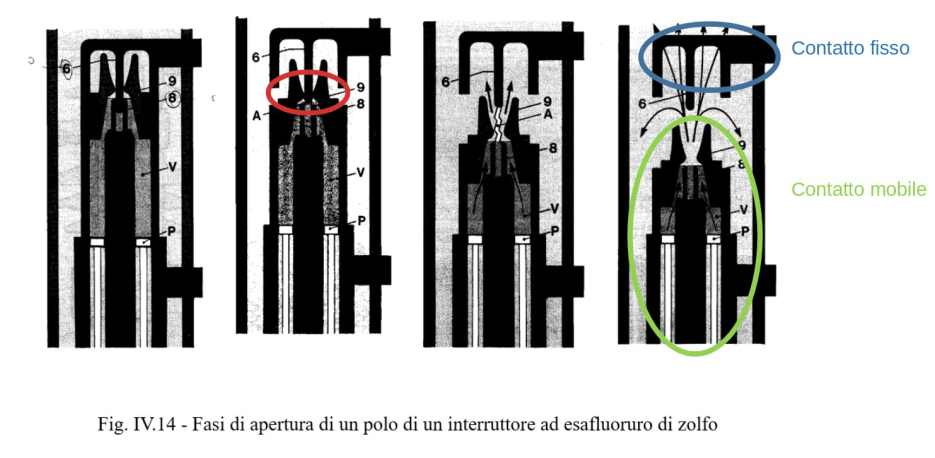
\includegraphics[width=0.8\linewidth]{immagini/manovra12}
\end{figure}

\begin{enumerate}
    \item Durante la traslazione del contatto mobile, un pistone fisso (P) comprime il gas $\text{SF}_6$ nella camera cilindrica (V).
    \item In una prima fase, il nucleo espanso dell'arco ostruisce la strozzatura della camera (ugello dielettrico): tale fenomeno, detto \textbf{effetto tappo}, blocca l'efflusso del gas determinando una sovrapressione proporzionale all'entità della corrente da interrompere (effetto di autoregolazione pneumatica della pressione).
    \item In prossimità del passaggio per lo zero della corrente, l'energia termica diminuisce e l'effetto tappo scompare: il gas compresso defluisce violentemente attraverso l'ugello investendo l'arco con un soffio assiale ad altissima velocità, deionizzando e raffreddando completamente lo spazio interelettrodico.
\end{enumerate}

\section{Sezionatori}
La funzione del sezionatore risponde alle esigenze di sicurezza degli operatori durante gli interventi di manutenzione, revisione, collaudo o modifica delle configurazioni di impianto. A tal fine deve soddisfare due vincoli:
\begin{enumerate}
    \item \textbf{Distanze minime di isolamento} $\rightarrow$ garantire in aria e lungo le superfici isolanti distanze sufficienti a escludere qualsiasi scarica tra i poli dell'apparecchio aperto.
    \item \textbf{Verifica certa dello stato di aperto} $\rightarrow$ consentire all'operatore di riscontrare la posizione di aperto in modo visivo diretto oppure tramite un dispositivo indicatore affidabile.
\end{enumerate}

I sezionatori non possiedono organi di spegnimento dell'arco e possono essere manovrati esclusivamente a circuito disalimentato o percorso da correnti di intensità trascurabile (come le correnti a vuoto di brevi tratti di barra o trasformatori di tensione).

Negli interventi su linee elettriche, sui conduttori possono permanere tensioni pericolose indotte o dovute a cariche residue elettrostatiche accumulate. Le norme impongono la messa a terra e in cortocircuito dei conduttori mediante \textbf{sezionatori di terra}. Questi dispositivi sono meccanicamente o elettricamente \textbf{interbloccati} (linee tratteggiate) con i corrispondenti sezionatori di linea in serie: l'interblocco impedisce la chiusura del sezionatore di terra se il sezionatore di linea è ancora chiuso, ed evita l'alimentazione accidentale di una linea posta a terra.
\begin{figure}[H]
	\centering
	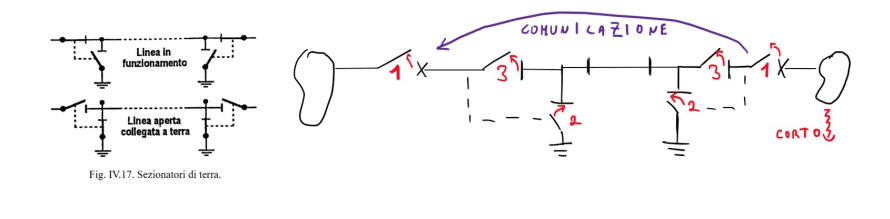
\includegraphics[width=1\linewidth]{immagini/manovra13}
\end{figure}

In base alla tipologia costruttiva, i sezionatori si suddividono in:
\begin{itemize}
    \item \textbf{Sezionatori a coltelli} $\rightarrow$ impiegati per impianti di I, II e III categoria.
    \item \textbf{Sezionatori a scorrimento assiale} $\rightarrow$ impiegati per impianti di II categoria.
    \item \textbf{Sezionatori a rotazione} $\rightarrow$ impiegati per impianti di II e III categoria.
    \item \textbf{Sezionatori a pantografo} $\rightarrow$ impiegati per impianti di III categoria (alta e altissima tensione).
    \item \textbf{Sezionatori a ginocchio} $\rightarrow$ impiegati per impianti di III categoria.
\end{itemize}
\begin{figure}[H]
	\centering
	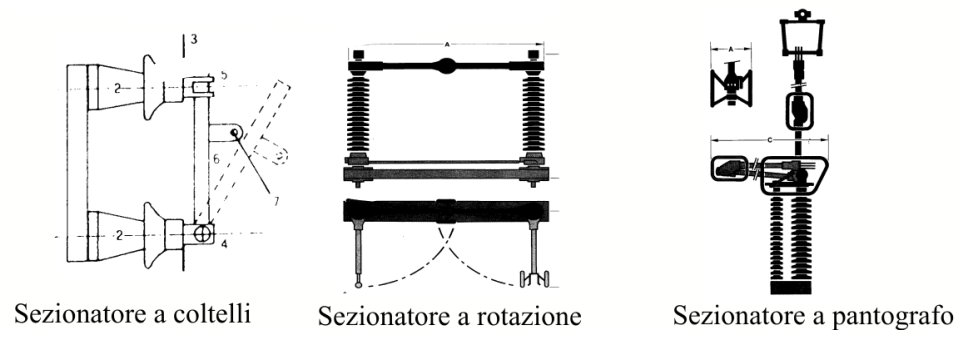
\includegraphics[width=0.7\linewidth]{immagini/manovra14}
\end{figure}

\section{Altri apparecchi di manovra e protezione}
\subsection{Interruttori di manovra e interruttori di manovra-sezionatori}
Gli interruttori di manovra presentano caratteristiche intermedie tra gli interruttori e i sezionatori:
\begin{itemize}
    \item Sono capaci di stabilire correnti sia in condizioni normali che su cortocircuito. Il loro \textbf{potere di chiusura} coincide con quello degli interruttori.
    \item Non sono in grado di interrompere le correnti di cortocircuito. Il loro \textbf{potere di interruzione} coincide con il valore efficace della massima corrente in condizioni normali (corrente nominale o modesti sovraccarichi) che possono estinguere.
\end{itemize}

Se integrano requisiti di visibilità e distanze di isolamento prescritte per la sicurezza, prendono il nome di \textbf{interruttori di manovra-sezionatori}. Vengono impiegati tipicamente per l'interruzione e la gestione di:
\begin{itemize}
    \item Carichi prevalentemente attivi.
    \item Circuiti di rete ad anello.
    \item Trasformatori funzionanti a vuoto.
    \item Batterie di condensatori.
    \item Linee aeree di modesta estensione e cavi a vuoto.
    \item Motori elettrici.
\end{itemize}

\subsection{Contattori}
A differenza degli altri apparecchi di manovra dotati di due posizioni meccanicamente stabili (aperto e chiuso), i contattori possiedono \textbf{una sola posizione di riposo}, tipicamente la posizione di circuito aperto. Il passaggio e la permanenza nello stato di chiuso avvengono unicamente tramite un comando continuo non manuale erogato da una sorgente energetica esterna (solitamente un elettromagnete ausiliario alimentato in tensione); al cessare dell'eccitazione della bobina, le molle di richiamo riportano istantaneamente l'apparecchio nella posizione di riposo aperto.

I contattori:
\begin{itemize}
    \item Possono stabilire e interrompere correnti esclusivamente in condizioni ordinarie di esercizio: il loro potere di apertura e di chiusura è riferito alla massima corrente normale.
    \item Presentano una resistenza all'usura da manovra eccezionalmente elevata, essendo capaci di sopportare centinaia di migliaia di cicli di apertura e chiusura senza degrado significativo dei contatti.
    \item Sono facilmente comandabili a distanza.
\end{itemize}

Per queste peculiarità, i contattori sono ampiamente impiegati in abbinamento agli interruttori per comandare assorbitori con manovre molto frequenti (motori, condensatori, reostati, lampade), salvaguardando l'interruttore da un logorio meccanico precoce.

È importante osservare che le Norme associano a ciascuna
categoria di utilizzazione ben precisi valori dei poteri di
interruzione e di chiusura, con la conseguenza che non è
necessario nei contattori indicare esplicitamente tali grandezze,
ma basta indicare la categoria di utilizzazione cui sono destinati.

\subsection{Fusibili}
Il fusibile è un dispositivo di protezione autonomo a ingombro e costo ridotti in grado di interrompere correnti di sovraccarico e di cortocircuito in media e bassa tensione.

Il principio si basa sull'interruzione fisica del percorso conduttivo mediante fusione per calore di un componente calibrato, denominato \textbf{elemento fusibile} (filo metallico o nastro sagomato in argento o rame con strozzature, immerso in sabbia di quarzo estinguente).
\begin{figure}[H]
	\centering
	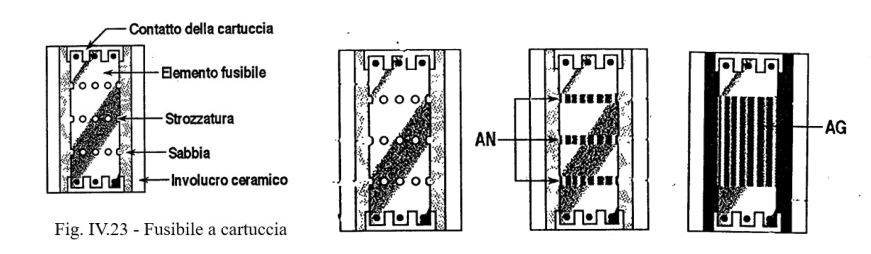
\includegraphics[width=0.75\linewidth]{immagini/manovra15}
\end{figure}

L'intervento è irreversibile e si articola in tre fasi temporali consecutive:
\begin{enumerate}
    \item \textbf{Fase di pre-arco (durata di pre-arco)} $\rightarrow$ la sovracorrente attraversa l'elemento fusibile; a causa dell'elevata densità di corrente nelle sezioni ristrette, il metallo si scalda fino alla temperatura di fusione ed evapora localmente.
    \item \textbf{Fase d'arco (durata d'arco)} $\rightarrow$ tra i lembi fusi dell'elemento scocca un arco elettrico che si propaga nella camera; la sabbia silicea fonde assorbendo calore dall'arco, vetrificando e deionizzando rapidamente il canale di scarica fino allo spegnimento.
    \item \textbf{Fase di post-arco} $\rightarrow$ l'arco è definitivamente estinto e lo spazio interrotto si assesta consolidando la resistenza dielettrica a circuito aperto.
\end{enumerate}
La somma della durata di pre-arco e della durata d'arco individua la \textbf{durata di interruzione} (o durata totale di funzionamento).

Un confronto tra fusibili e interruttori automatici evidenzia i seguenti vantaggi dei fusibili:
\begin{itemize}
    \item Costo di acquisto ridotto e ingombro volumetrico contenuto.
    \item Potere di interruzione molto elevato, virtualmente illimitato per gli impianti di I categoria.
    \item Altissima affidabilità intrinseca di scatto al cortocircuito, esente dai rischi di incollaggio meccanico o mancata manutenzione che possono affliggere gli interruttori.
\end{itemize}

I principali svantaggi comprendono:
\begin{itemize}
    \item Irreversibilità dell'intervento: ogni evento di fusione richiede la sostituzione fisica della cartuccia per il ripristino dell'alimentazione, a differenza dell'interruttore che richiede una semplice manovra di richiusura.
    \item Rischio di marcia a due fasi: nelle linee trifasi a monte di motori, la fusione del fusibile su una sola fase a seguito di un guasto monofase lascia attive le altre due fasi, provocando pericolosi squilibri e gravi surriscaldamenti negli avvolgimenti delle macchine rotanti.
    \item Incapacità di compiere manovre ordinarie a vuoto o sotto carico: i fusibili reagiscono esclusivamente a sovracorrenti e devono pertanto essere associati in serie a un apparecchio di manovra separato (es. sezionatore o interruttore di manovra-sezionatore).
\end{itemize}

\subsection{Quadro di sintesi per categoria di tensione}
L'impiego dei diversi apparecchi di manovra si articola nelle reti in base alla classe di tensione dell'impianto:
\begin{itemize}
    \item \textbf{Sistemi di I Categoria (Bassa Tensione)}:
    \begin{itemize}
        \item Interruttori in aria.
        \item Sezionatori a coltelli.
        \item Interruttori di manovra-sezionatori.
        \item Contattori.
        \item Fusibili.
    \end{itemize}
    \item \textbf{Sistemi di II Categoria (Media Tensione)}:
    \begin{itemize}
        \item Interruttori in aria a soffio magnetico, a volume d'olio ridotto, in aria compressa, in esafluoruro di zolfo ($\text{SF}_6$), sotto vuoto.
        \item Sezionatori a coltelli, a rotazione, a scorrimento assiale.
        \item Interruttori di manovra-sezionatori.
        \item Fusibili.
    \end{itemize}
    \item \textbf{Sistemi di III e IV Categoria (Alta e Altissima Tensione)}:
    \begin{itemize}
        \item Interruttori a volume d'olio ridotto, in aria compressa, in esafluoruro di zolfo ($\text{SF}_6$).
        \item Sezionatori a coltelli, a rotazione, a pantografo, a ginocchio.
    \end{itemize}
\end{itemize}

\section{Relè di protezione}
Il relè costituisce l'organo sensibile e intelligente del sistema di protezione: controlla grandezze fisiche rappresentative dello stato della rete (corrente, tensione, frequenza, temperatura, sfasamento) e comanda lo sgancio o l'apertura dell'apparecchio di manovra non appena il parametro monitorato oltrepassa le soglie ammesse di sicurezza.

I relè di protezione non sono collegati direttamente ai circuiti ad alta o media tensione del sistema di potenza, ma vengono alimentati attraverso trasformatore di misura: \textbf{trasformatori di corrente (TA)} e \textbf{trasformatori di tensione (TV)}.

I trasformatori di misura adempiono a due funzioni imprescindibili:
\begin{enumerate}
    \item \textbf{Riduzione a valori secondari unificati} $\rightarrow$ riducono le elevate correnti e tensioni di rete a livelli compatibili con la circuiteria standardizzata dei relè (valori tipici normalizzati: $5\text{ A}$ o $1\text{ A}$ per i TA; $100\text{ V}$ o $100/\sqrt{3}\text{ V}$ per i TV).
    \item \textbf{Isolamento galvanico} $\rightarrow$ separano galvanicamente il circuito secondario di misura e protezione dalla rete primaria in alta/media tensione, garantendo l'incolumità del personale addetto e la sicurezza degli strumenti.
\end{enumerate}

Sotto il profilo circuitale, la rete di potenza agisce da generatore ideale collegato all'avvolgimento primario del trasformatore di misura, mentre il circuito d'ingresso del relè funge da carico collegato ai morsetti del secondario.
\begin{figure}[H]
	\centering
	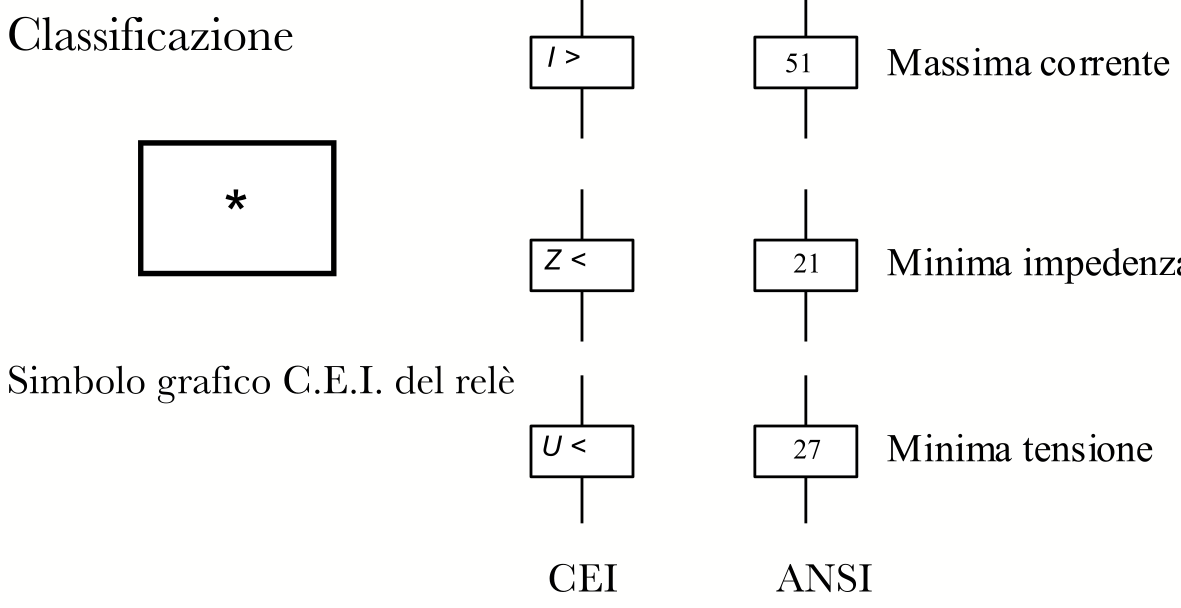
\includegraphics[width=0.6\linewidth]{immagini/manovra16}
\end{figure}

I relè si classificano secondo molteplici criteri funzionali e costruttivi:
\begin{figure}[H]
	\centering
	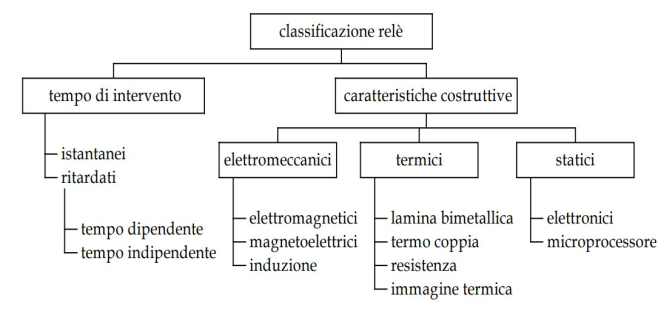
\includegraphics[width=0.7\linewidth]{immagini/manovra18}
\end{figure}
\begin{itemize}
    \item \textbf{In base alla natura del principio costruttivo}:
    \begin{itemize}
        \item \emph{Elettromeccanici}: basati sullo spostamento relativo di organi meccanici sotto l'azione di coppie o forze generate da correnti (a elettromagnete, a magnetoelettrici, a induzione).
        \item \emph{Termici}: basati sulla deformazione termomeccanica o sulla variazione di parametri per riscaldamento (a lamina bimetallica, a termocoppia, a resistenza, a immagine termica).
        \item \emph{Statici ed elettronici}: basati su circuiti a semiconduttore analogici, schede elettroniche digitali e architetture a microprocessore.
    \end{itemize}
    \item \textbf{In base al tempo di intervento}:
    \begin{figure}[H]
    	\centering
    	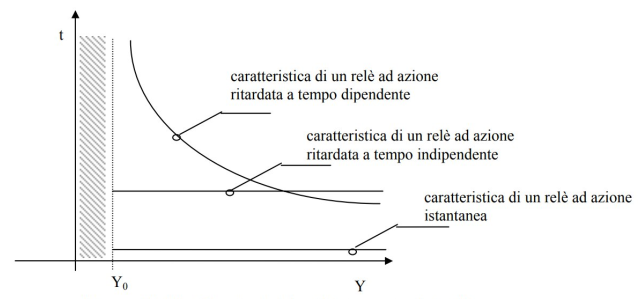
\includegraphics[width=0.6\linewidth]{immagini/manovra17}
    \end{figure}
    \begin{itemize}
        \item \emph{Istantanei}: l'ordine di scatto viene inviato senza alcun ritardo intenzionale non appena la grandezza sorpassa la soglia di regolazione ($Y > Y_0$).
        \item \emph{Ritardati}: il comando di scatto è ritardato nel tempo rispetto all'istante di superamento della soglia:
        \begin{itemize}
            \item \emph{A tempo indipendente (tempo costante)} $\rightarrow$ il ritardo di intervento $t$ è prefissato e costante, indipendente dall'entità del superamento del valore di soglia.
            \item \emph{A tempo dipendente (tempo inverso)} $\rightarrow$ il tempo di ritardo diminuisce al crescere dell'ampiezza della grandezza controllata ($t \propto 1/Y^\alpha$).
        \end{itemize}
    \end{itemize}
\end{itemize}

\subsection{Relè termico a lamina bimetallica}
Viene inserito in serie al carico per proteggere i circuiti dalle correnti di sovraccarico. È costituito da due lamine di metalli differenti saldate tra loro, aventi coefficienti di dilatazione termica sensibilmente disuguali.
\begin{figure}[H]
	\centering
	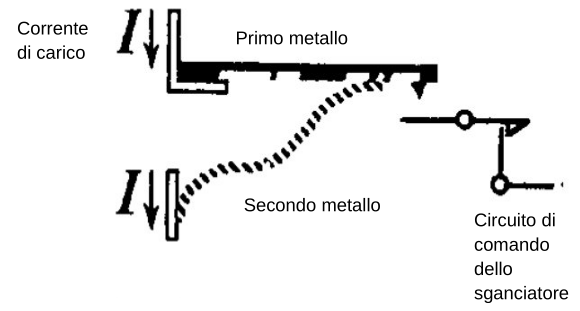
\includegraphics[width=0.4\linewidth]{immagini/manovra19}
\end{figure}
\begin{itemize}
    \item Quando la corrente di carico o di sovraccarico fluisce nella lamina, la temperatura cresce per effetto Joule.
    \item La differente espansione termica dei due metalli costringe la barra ad arcuarsi verso il metallo a minore coefficiente di dilatazione.
    \item Al raggiungimento di una determinato livello di deformazione, la lamina preme sul cinematismo di scatto aprendo il circuito di comando dello sganciatore dell'interruttore.
    \begin{figure}[H]
    	\centering
    	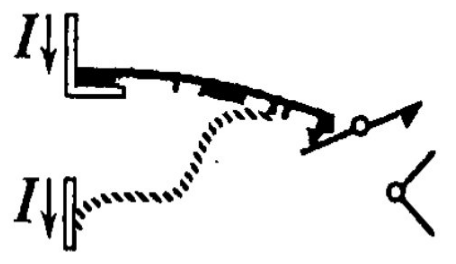
\includegraphics[width=0.25\linewidth]{immagini/manovra20}
    \end{figure}
    \item È una protezione tipicamente \textbf{a tempo dipendente}: l'energia termica accumulata dipende dall'integrale $\int i^2 dt$, per cui una corrente di sovraccarico debole richiede tempi lunghi per innescare lo scatto, mentre un sovraccarico consistente induce una deformazione rapida.
    \begin{figure}[H]
    	\centering
    	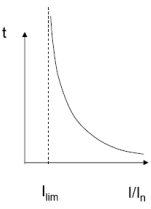
\includegraphics[width=0.2\linewidth]{immagini/manovra23}
    \end{figure}
    \item Cessata la circolazione di sovracorrente, la lamina si raffredda tornando spontaneamente alla configurazione geometrica originaria.
\end{itemize}

\subsection{Relè magnetico}
È un dispositivo sensibile alle correnti intense di cortocircuito, inserito in serie al circuito.

È costituito da un solenoide percorso dalla corrente di linea e da un'armatura ferromagnetica mobile trattenuta da una molla di forza calibrata $F_M$.
\begin{figure}[H]
	\centering
	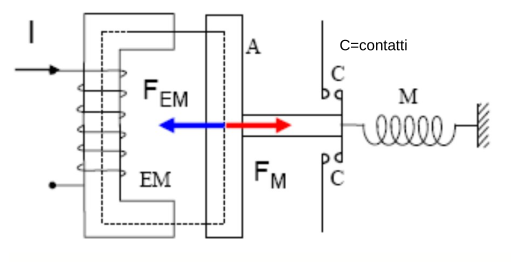
\includegraphics[width=0.45\linewidth]{immagini/manovra21}
\end{figure}
In condizioni di corrente nominale, il flusso magnetico genera una forza di attrazione elettromagnetica inferiore alla reazione della molla ($F_{EM} < F_M$), e i contatti ausiliari rimangono aperti.

All'innesco di una corrente di cortocircuito, la forza di richiamo magnetico cresce repentinamente vincendo la forza elastica ($F_{EM} > F_M$): l'armatura si serra istantaneamente azionando i contatti che pilotano la bobina di apertura dell'interruttore.

È una protezione tipicamente \textbf{istantanea} o associabile a un temporizzatore a tempo indipendente.
\begin{figure}[H]
	\centering
	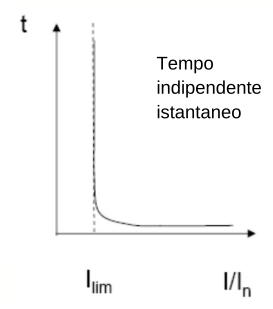
\includegraphics[width=0.3\linewidth]{immagini/manovra22}
\end{figure}

\subsection{Relè magneto-termico}
Integra in un unico corpo compatto le funzionalità del relè termico e del relè magnetico:
\begin{itemize}
    \item La lamina bimetallica garantisce la protezione contro le deboli correnti di sovraccarico prolungate a tempo inverso.
    \item Il solenoide ad attrazione rapida garantisce la protezione istantanea ad alta velocità contro le correnti violente di cortocircuito.
\end{itemize}
\begin{figure}[H]
	\centering
	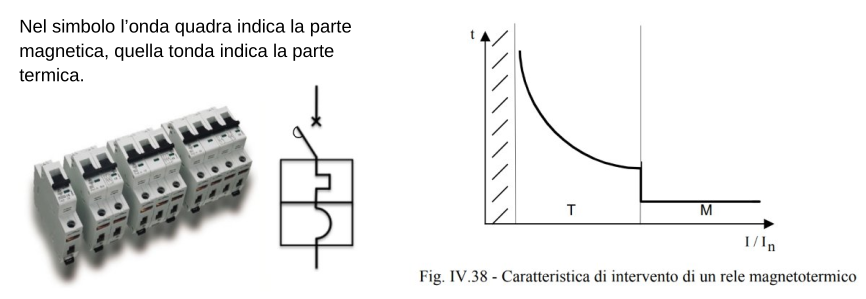
\includegraphics[width=0.7\linewidth]{immagini/manovra24}
\end{figure}
La curva di intervento complessiva risultante nel piano tempo-corrente $(t - I)$ è data dalla combinazione della caratteristica iperbolica del termico per correnti comprese tra $I_n$ e la soglia magnetica, raccordata alla linea verticale istantanea del magnetico per correnti superiori. Nei simboli unifilari normalizzati, la funzione magnetica è denotata da un profilo rettangolare/a gradino, mentre la funzione termica è identificata da un profilo curvilineo.
\begin{figure}[H]
	\centering
	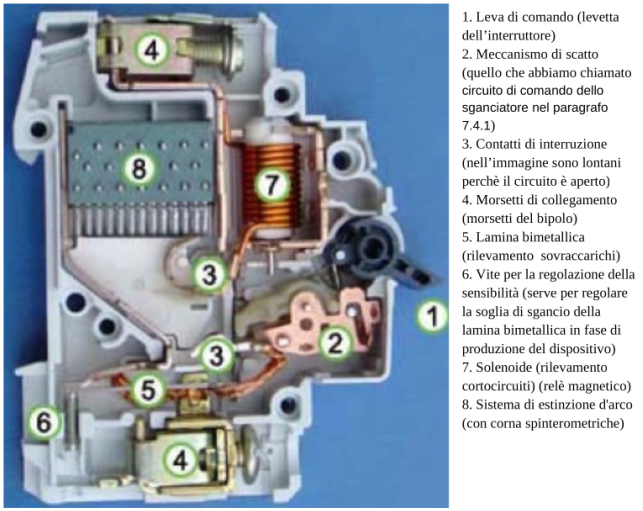
\includegraphics[width=0.8\linewidth]{immagini/manovra25}
\end{figure}


\subsection{Relè differenziale}
Il relè differenziale è il dispositivo primario deputato alla protezione delle persone contro i contatti indiretti e alla rilevazione delle correnti di dispersione verso terra negli impianti di I categoria.
\begin{figure}[H]
	\centering
	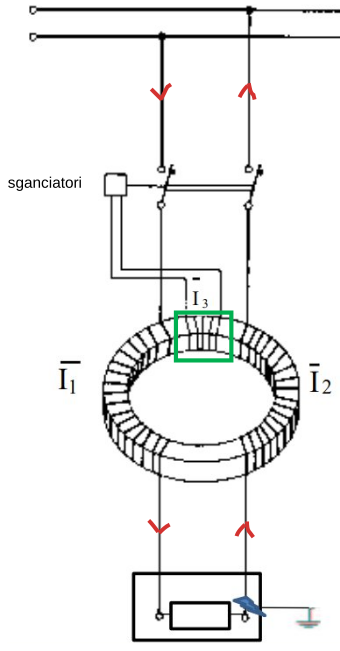
\includegraphics[width=0.3\linewidth]{immagini/manovra26}
\end{figure}
Il principio si basa sul bilancio vettoriale delle correnti:
\begin{itemize}
    \item I conduttori attivi di alimentazione (fase e neutro nel monofase, o le tre fasi più l'eventuale neutro nel trifase) sono avvolti, in verso opposto, attorno ad un toroide ad elevata permeabilità.
    \item In condizioni di normali, la somma istantanea delle correnti è nulla:
    \[\sum_{k} i_k(t) = 0\]
    I flussi magnetici elementari generati dai singoli conduttori nel toroide si compensano reciprocamente e il flusso risultante nel nucleo è nullo ($\Phi_{tot} = 0$).
    \item In presenza di un guasto a terra o di contatto accidentale, una quota di corrente ($i_d$) si disperde verso il terreno o l'involucro metallico senza fare ritorno attraverso i conduttori attivi.
    \item Si genera un flusso magnetico netto nel nucleo toroide proporzionale a $i_d$. Tale flusso induce una forza elettromotrice su un avvolgimento secondario ausiliario avvolto sul toro, il quale alimenta una bobina di sgancio.
\end{itemize}
\begin{figure}[H]
	\centering
	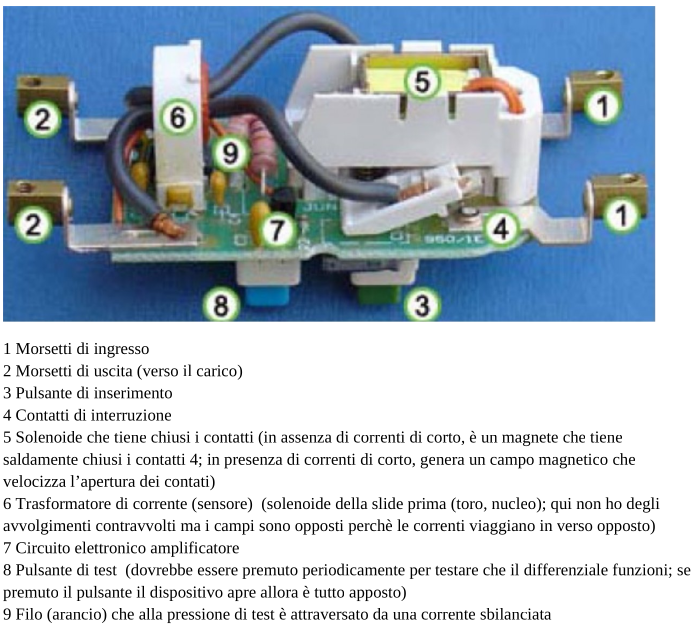
\includegraphics[width=0.7\linewidth]{immagini/manovra27}
\end{figure}

\subsubsection{Tipologie di differenziali}
\begin{itemize}
    \item \textbf{Tipo AC} $\rightarrow$ differenziali tradizionali idonei a intervenire esclusivamente in presenza di correnti differenziali di guasto alternate sinusoidali, applicate improvvisamente o lentamente crescenti (adatti a carichi domestici lineari resistivi).
    \item \textbf{Tipo A} $\rightarrow$ assicurano l'intervento sia per correnti sinusoidali alternate, sia in presenza di correnti unidirezionali pulsanti (generate da carichi raddrizzatori a diodi o tiristori, azionamenti elettronici, elettrodomestici inverter).
    \item \textbf{Tipo S (Selettivi)} $\rightarrow$ differenziali ritardati intenzionalmente nel tempo di scatto (ritardo fisso o tarabile) rispetto ai differenziali standard; vengono installati come interruttori generali a monte per consentire la selettività differenziale cronometrica con i dispositivi istantanei posti a valle.
\end{itemize}
\begin{figure}[H]
	\centering
	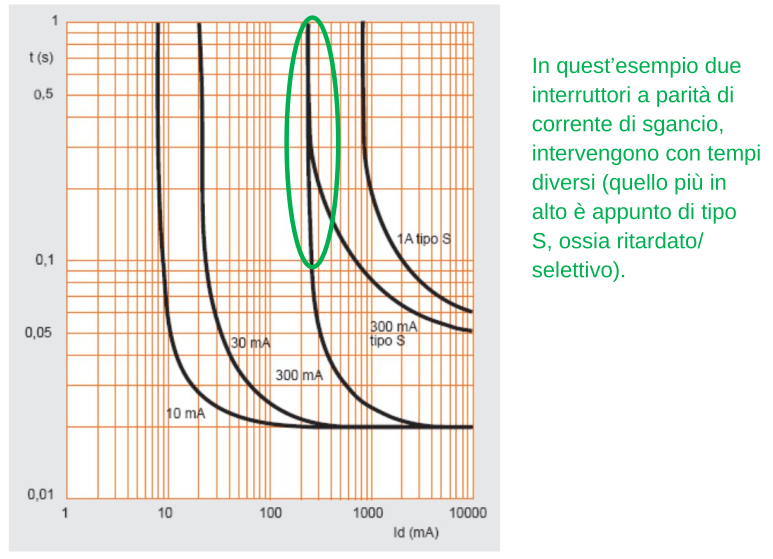
\includegraphics[width=0.6\linewidth]{immagini/manovra28}
\end{figure}
